
\documentclass[dvipsnames]{article}
\usepackage{amsmath}
\usepackage{amssymb}
\usepackage{bm}
\usepackage{fancybox, graphicx}
\usepackage{tikz} % Diagrams
\usepackage{color}

\usepackage{geometry}
\geometry{a3paper, margin=0.3cm}


\begin{document}

\pagenumbering{gobble} % No page number

\begin{figure}
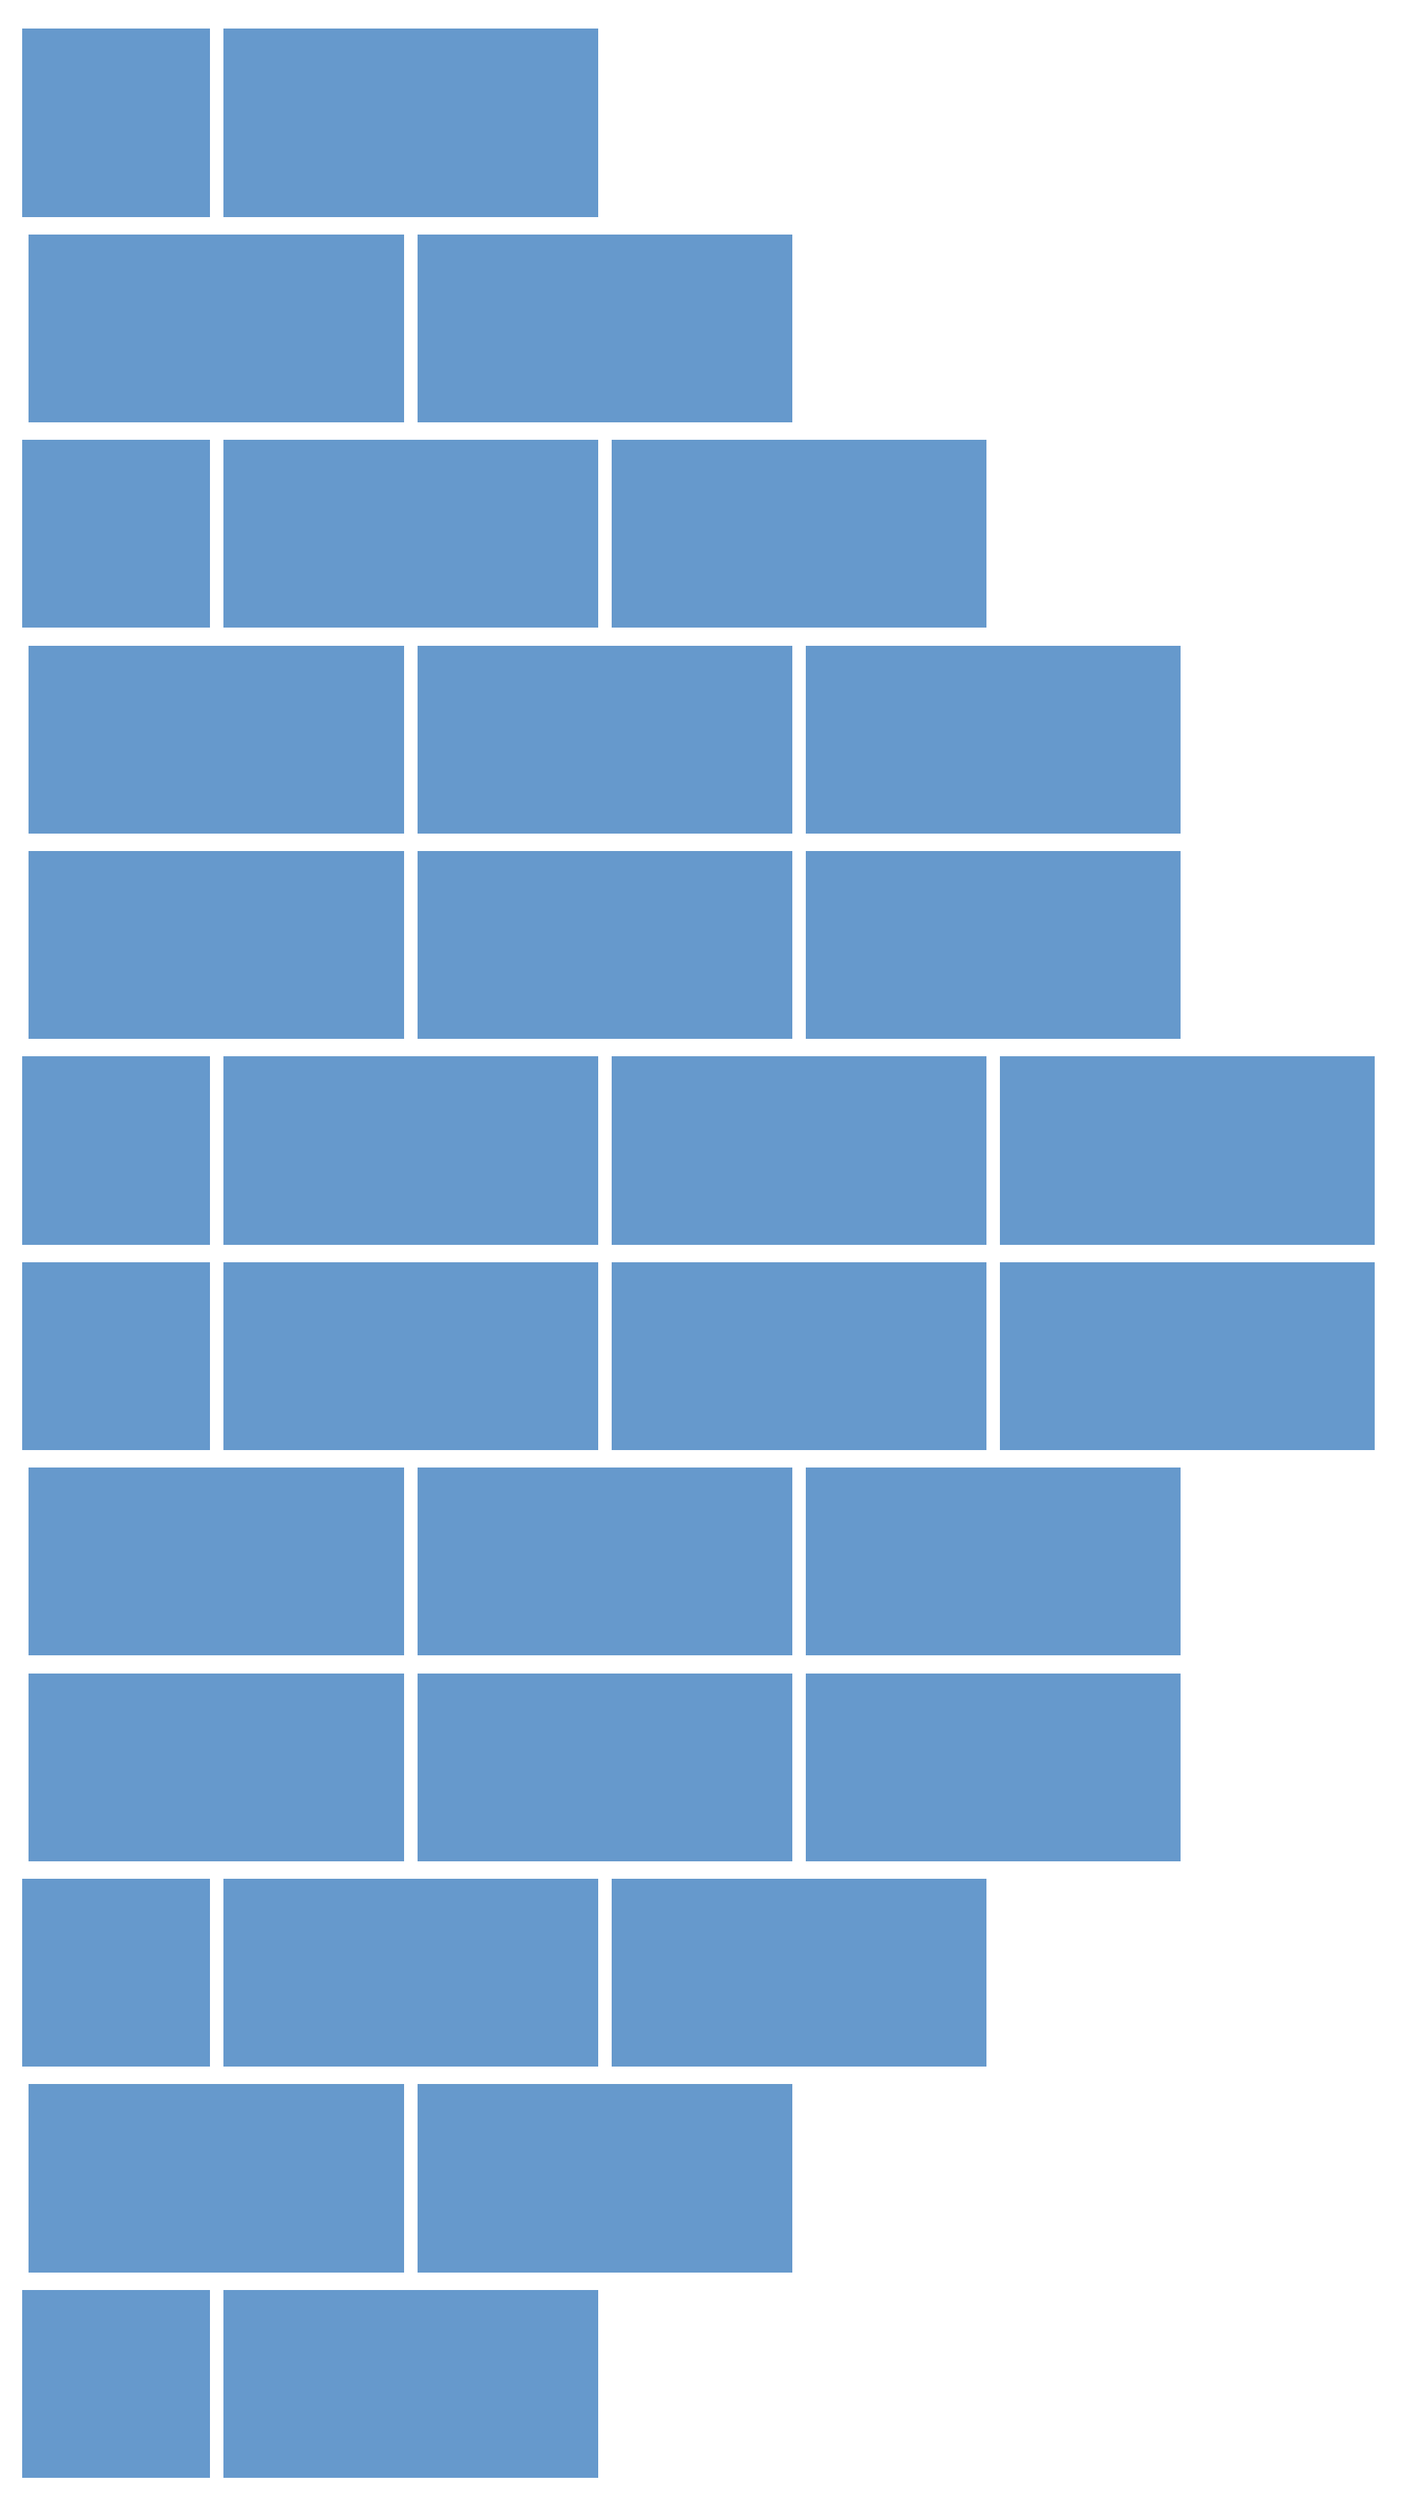
\begin{tikzpicture}[font=\ttfamily]
\definecolor{bluegray}{rgb}{0.4, 0.6, 0.8} % From http://latexcolor.com/

% The following text was automatically generated using code in DECamCCDLayout.py.
% Do not edit! Change the Python code instead.

\draw  [fill=bluegray,bluegray] (0.000,1.758) rectangle (3.000,4.758) node {};
\draw  [fill=bluegray,bluegray] (3.224,1.758) rectangle (9.224,4.758) node {};
\draw  [fill=bluegray,bluegray] (0.112,5.052) rectangle (6.112,8.052) node {};
\draw  [fill=bluegray,bluegray] (6.336,5.052) rectangle (12.336,8.052) node {};
\draw  [fill=bluegray,bluegray] (0.000,8.347) rectangle (3.000,11.347) node {};
\draw  [fill=bluegray,bluegray] (3.224,8.347) rectangle (9.224,11.347) node {};
\draw  [fill=bluegray,bluegray] (9.448,8.347) rectangle (15.448,11.347) node {};
\draw  [fill=bluegray,bluegray] (0.112,11.641) rectangle (6.112,14.641) node {};
\draw  [fill=bluegray,bluegray] (6.336,11.641) rectangle (12.336,14.641) node {};
\draw  [fill=bluegray,bluegray] (12.560,11.641) rectangle (18.560,14.641) node {};
\draw  [fill=bluegray,bluegray] (0.112,14.936) rectangle (6.112,17.936) node {};
\draw  [fill=bluegray,bluegray] (6.336,14.936) rectangle (12.336,17.936) node {};
\draw  [fill=bluegray,bluegray] (12.560,14.936) rectangle (18.560,17.936) node {};
\draw  [fill=bluegray,bluegray] (0.000,18.230) rectangle (3.000,21.230) node {};
\draw  [fill=bluegray,bluegray] (3.224,18.230) rectangle (9.224,21.230) node {};
\draw  [fill=bluegray,bluegray] (9.448,18.230) rectangle (15.448,21.230) node {};
\draw  [fill=bluegray,bluegray] (15.672,18.230) rectangle (21.672,21.230) node {};
\draw  [fill=bluegray,bluegray] (0.000,21.524) rectangle (3.000,24.524) node {};
\draw  [fill=bluegray,bluegray] (3.224,21.524) rectangle (9.224,24.524) node {};
\draw  [fill=bluegray,bluegray] (9.448,21.524) rectangle (15.448,24.524) node {};
\draw  [fill=bluegray,bluegray] (15.672,21.524) rectangle (21.672,24.524) node {};
\draw  [fill=bluegray,bluegray] (0.112,24.819) rectangle (6.112,27.819) node {};
\draw  [fill=bluegray,bluegray] (6.336,24.819) rectangle (12.336,27.819) node {};
\draw  [fill=bluegray,bluegray] (12.560,24.819) rectangle (18.560,27.819) node {};
\draw  [fill=bluegray,bluegray] (0.112,28.113) rectangle (6.112,31.113) node {};
\draw  [fill=bluegray,bluegray] (6.336,28.113) rectangle (12.336,31.113) node {};
\draw  [fill=bluegray,bluegray] (12.560,28.113) rectangle (18.560,31.113) node {};
\draw  [fill=bluegray,bluegray] (0.000,31.408) rectangle (3.000,34.408) node {};
\draw  [fill=bluegray,bluegray] (3.224,31.408) rectangle (9.224,34.408) node {};
\draw  [fill=bluegray,bluegray] (9.448,31.408) rectangle (15.448,34.408) node {};
\draw  [fill=bluegray,bluegray] (0.112,34.702) rectangle (6.112,37.702) node {};
\draw  [fill=bluegray,bluegray] (6.336,34.702) rectangle (12.336,37.702) node {};
\draw  [fill=bluegray,bluegray] (0.000,37.997) rectangle (3.000,40.997) node {};
\draw  [fill=bluegray,bluegray] (3.224,37.997) rectangle (9.224,40.997) node {};

% End of automatically-generated text
\end{tikzpicture}
\end{figure}


\end{document}
